\chapter{Motivation \& Outline}\label{motivation}

The goal of this thesis is to create a network that can be used to gain insight into the causes of side effects for a given drug relying on the relationships between chemicals, targets, phenotypes (Figure~\ref{fig:triangle}).
In which case, the cause of side effects can be understood by analyzing the mechanism of action of drugs.

\begin{figure}[!ht]
    \centering
    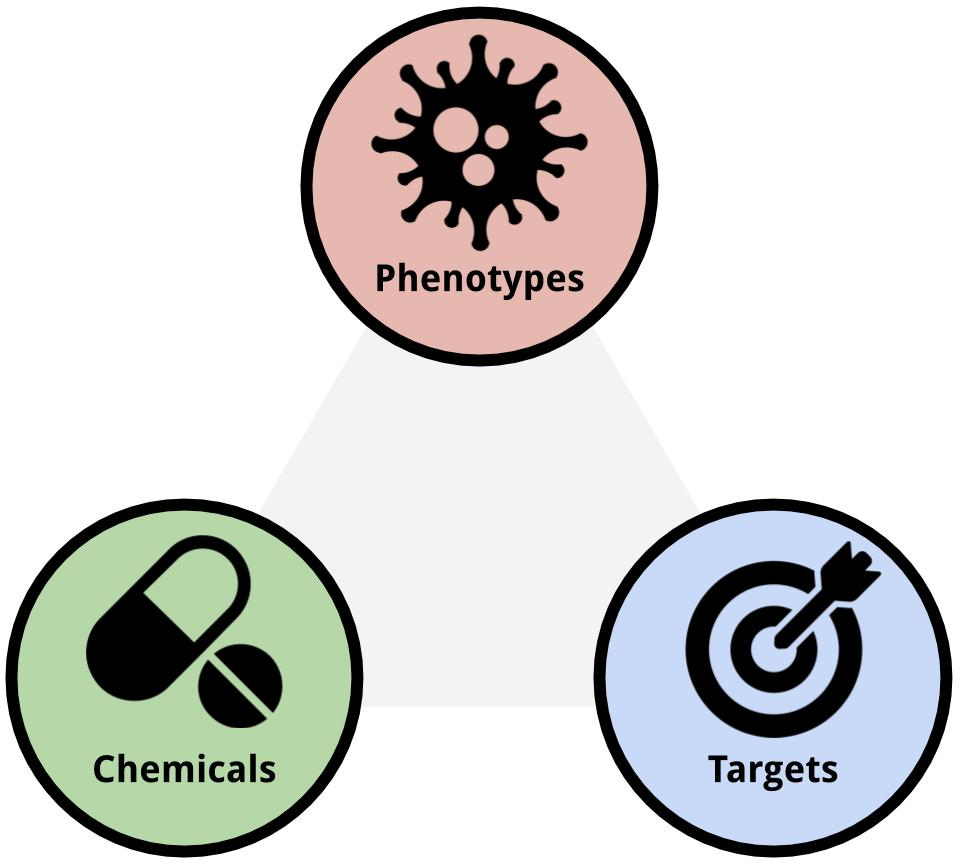
\includegraphics[scale=0.175]
    {figures/triangle.jpg}
    \captionsetup{justification=centering}
    \caption{\label{fig:triangle} Chemicals-targets-phenotypes relationship triangle.}
\end{figure}

To achieve the goals of the project, first, a knowledge graph was created and enriched from multiple sources.
This graph contained three different types of entities:chemicals, targets, and phenotypes.
It contained three different relations: chemical-chemical, chemical-target and chemical-phenotype.
Various \ac{NRL} approaches were used to create embeddings of the graph, which were then trained and optimized to obtain the best predictive model.
This model was used to predict new relations with different node types, which were then contextualized with additional literature.
A schematic of the workflow is presented in Figure~\ref{fig:workflow}.

\begin{figure}[!ht]
    \centering
    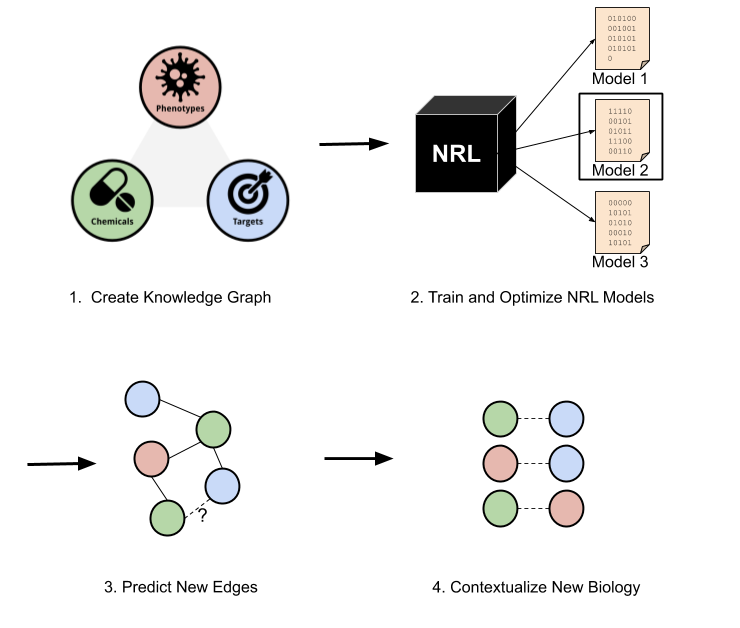
\includegraphics[scale=0.60]
    {figures/workflow.png}
    \captionsetup{justification=centering}
    \caption{\label{fig:workflow} The workflow of this thesis.}
\end{figure}
